\section{Application programming model}
\label{Concept}
\label{Concept:APM}

Applications are required to implement a specific programming model in order to make full use of the accelerator scheduling kernel extension. We made this design choice since the scheduler needs a method to pass the control of a processing unit to a specific task, but the NVIDIA CUDA runtime so far only provides a first-come-first-serve scheduler. As the CUDA libraries are closed source, the only way to ensure that only a scheduled task is allowed to execute would be a library wrapper for them. This wrapper would have to communicate with the CUDA libraries and could hence not be fully integrated into the kernel. A daemon in user space would be necessary since it additionally would have to react to the scheduling decisions of the extension. As the user space side was only of interest for evaluation purposes and not the focal point of this approach, we decided against the user space daemon in favor of a more simple but still effective programming model which employs cooperative multitasking. This model will be detailed in the remainder of this section.

As threads are our schedulable entities they also are the scope of our model. Chapter~\ref{Implementation} will give an overview over one possible integration of this concept into a complete application. Applying the model to a thread creates a task which communicates with the scheduler extension, allowing the operating system to administer the usage of its heterogeneous \cus{}. We will call such a task a ``hardware task'' in this document. It has to provide an implementation of its main algorithm for one or more architectures in the corresponding binary format and has to invoke the code designed for the unit which the extension assigns to it. Every actual communication with the devices themselves has to be done by this task, since the libraries needed to perform that communication are at least in the case of NVIDIA GPUs closed source user space libraries. We call the administrative part of the hardware task its ``ghost thread''. If the scheduler assigns a CPU core to a hardware task, the differentiation between the computational part and the ghost thread is merely of organizational nature, as both parts will mostly be performed by the same thread. In the case of hardware accelerators however the ghost thread is the part which has to be run on a CPU, i.e. the part that executes the system calls, branches to the correct device code, performs the memory management and copies the data to and from the device, invokes the computational part on the accelerator and waits for its completion. The name ``ghost thread'' stems from this list of activities, as it is a shadow representative of the accelerator code, which the scheduler can manipulate and schedule. It does not stress the CPU on which it is executed, because it primarily carries out blocking I/O functions, and thus waits most of the time.

An existing application can source out every part that is acceleratable to a hardware task. This is not limited to parallel computations, since the ghost threads are standard POSIX threads, and hence the program may wait for them to finish before proceeding, or synchronize with them in any other standard way. If it provides CPU and NVIDIA CUDA implementations, a program augmented with hardware tasks would be able to run on a system with or without a CUDA card, without change to the program. Two such programs could run in a system with one card using an interleaving execution pattern on the unit, orchestrated by the scheduler extension. This time sharing would allow for continuous accessibility of the accelerator from the users point of view, and could increase the possible interactivity of both programs.

Figure~\ref{fig:FlowDiaHWT} displays the program flow of a hardware task. The steps in which data or code is copied or such resources are released, only apply to accelerators and may be skipped for execution on a CPU. Analogously, while the ghost threads actually wait in a blocked state for the accelerator to reach the next checkpoint, they have to perform the calculation steps to reach that checkpoint if the assigned unit is a CPU.
\begin{figure}[htbp]
  \centering
    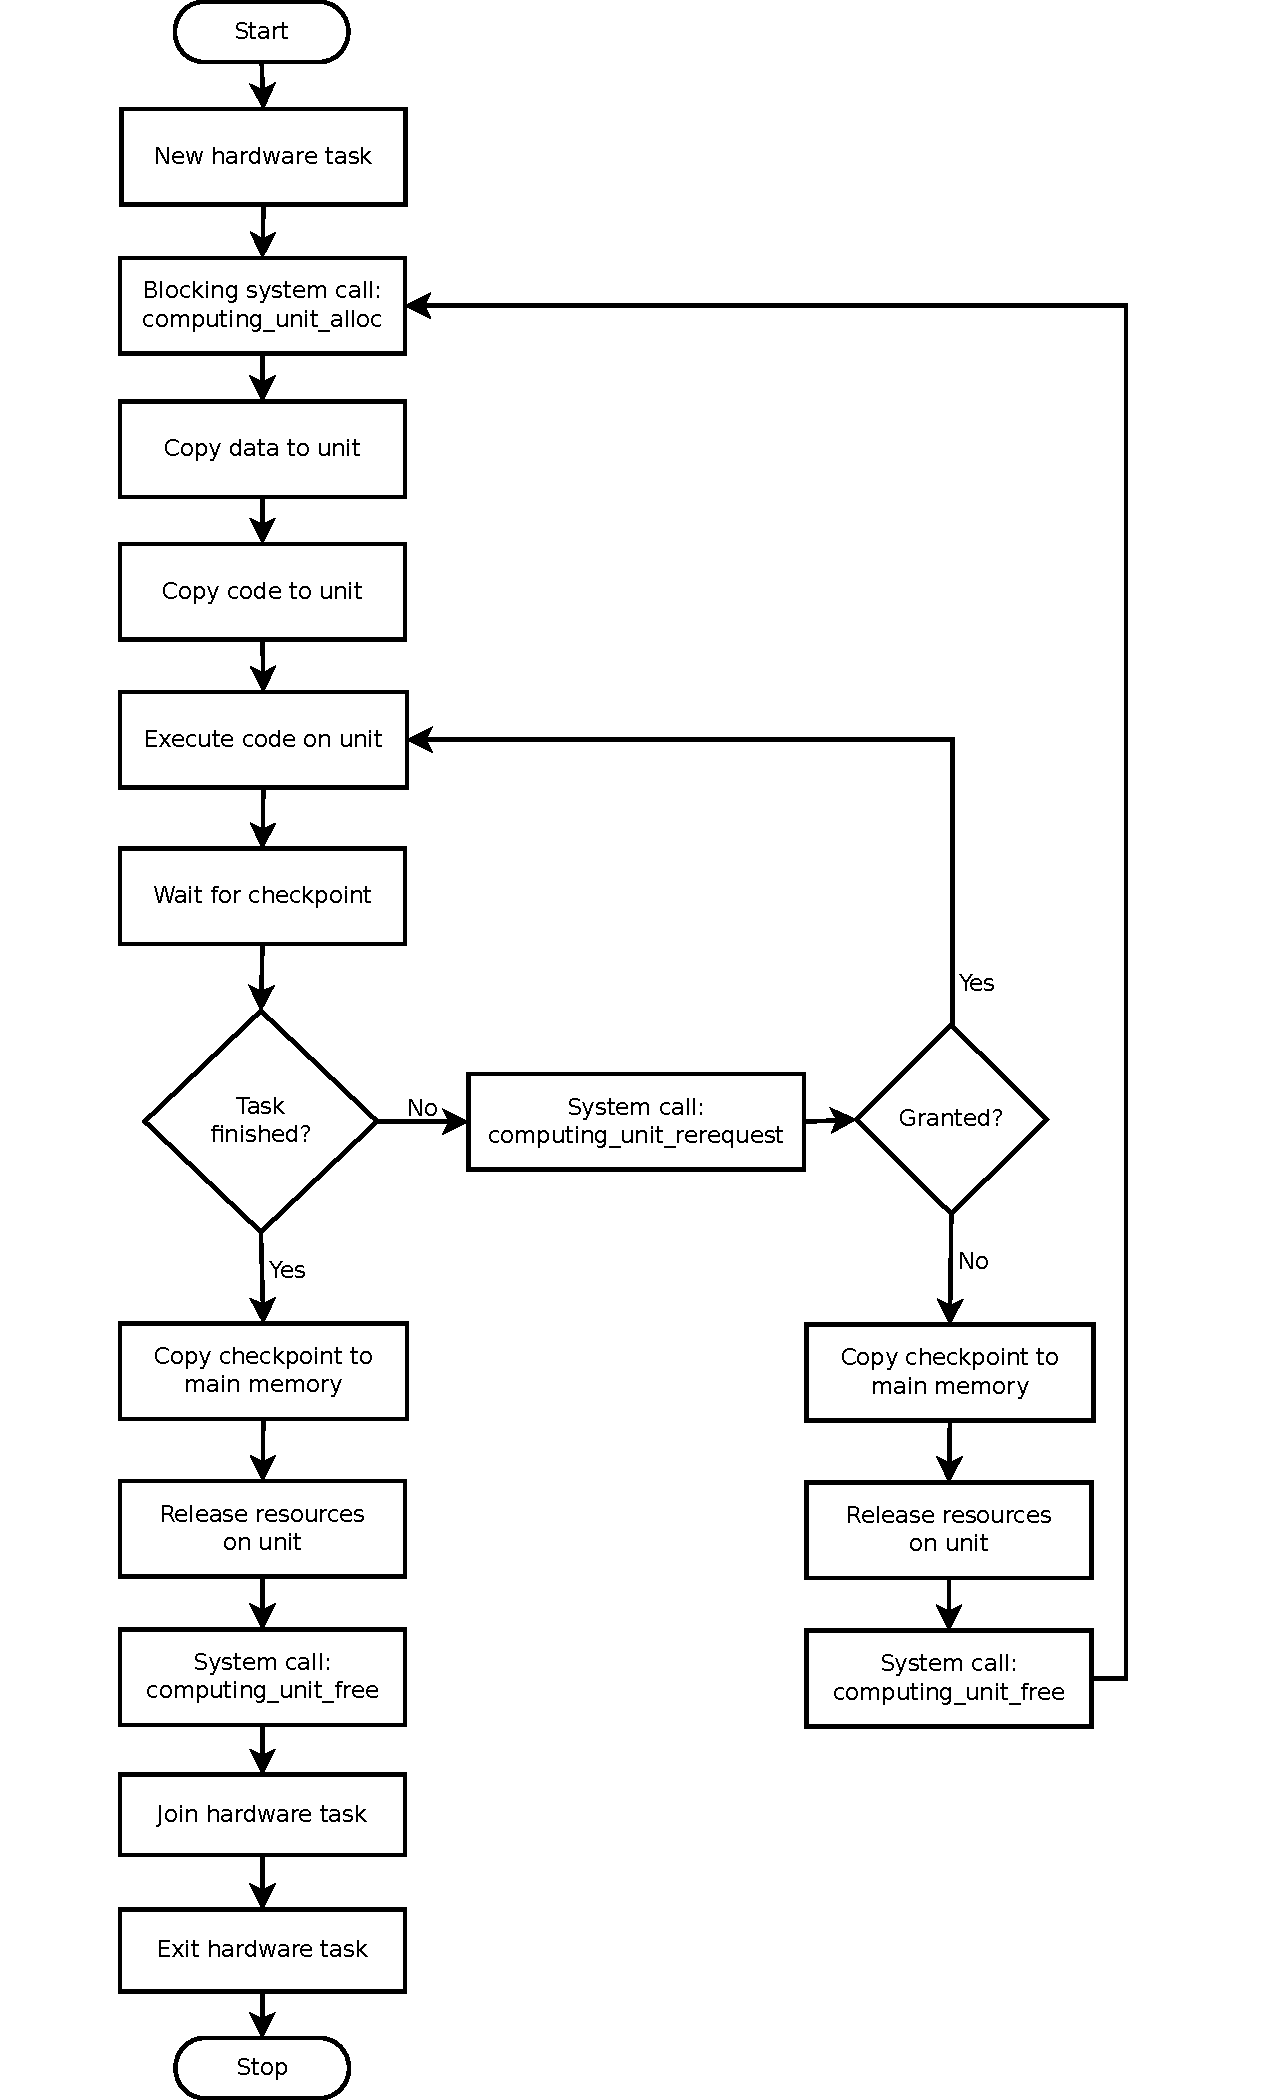
\includegraphics[width=0.90\textwidth]{FD_hardware_task}
  \caption[Program flow of a Hardware Task]{Program flow of a hardware task.}
  \label{fig:FlowDiaHWT}
\end{figure}
After being created by its parent task, a hardware task has to allocate a \cu{} using the \functionname{allocation} system call of the scheduler extension. This call blocks until a valid resource could be found or fails if there are no suitable devices present in the system. Should the call return, the hardware task may allocate memory on the assigned device and copy its data to it. This may be a checkpoint from a previous run or just constant or initial data. Afterwards it should copy the binary with the device code to the resource and start the execution. If the assigned unit is a CPU then the hardware task actually performs the computation itself here, or it starts a delegate thread for that purpose. If either a new checkpoint has been reached or the task has finished all calculations, the execution returns. If the task has not finished its work and can continue to use the last assigned accelerator, it should re-request the unit from the kernel extension, as all needed computing resources are still on it. The scheduler may then grant or deny that request. Should it allow the further occupation of the unit, the task executes the code again to advance to the next checkpoint (or the end). If either the re-request has been denied or if the task has reached the last checkpoint, the hardware task has to copy the current checkpoint from the resource to main memory. Afterwards all allocated memory regions on the device have to be released. To signal the scheduler that it completely left the device, it then has to call the \functionname{free} routine of the extension. In case of a denied re-request the task can afterwards invoke the \functionname{allocation} call again, to request access to the same or another resource. If the task was done, it can be joined in the parent thread before exiting, using conventional threading methods.

The application may only copy data from or to and execute on a device which has been assigned to it via the \functionname{computing\_unit\_alloc} call. The assignment mechanism can therefore be seen as a locking technique not unlike a semaphore, where a hardware task has exclusive access to a computing unit between the system calls \functionname{computing\_unit\_alloc} and \functionname{computing\_unit\_free}.

There are two new structures defined in the kernel extension, which are needed for the \functionname{allocation} system call. They are defined in a public header file that can be embedded in applications.
The first of them is \codesnippet{struct meta\_info} and is defined as shown in Listing~\ref{lst:meta_info}, which has been reduced to key components. The field \codesnippet{memory\_to\_copy} denotes the amount of memory which has to be transferred to and from the device, and will obviously not be considered if the task is currently working on a CPU, as the checkpoint does not need to be copied in that case. Using this information together with the bandwidth of the device, the scheduler can estimate the time it will take to perform a task switch to or from this task. Hence this value is integrated into the individual scheduling granularity for this task. The \codesnippet{parallel\_efficiency\_gain} has to be estimated by the software developer on an arbitrary scale from $0$ to $5$. It should roughly reflect how much the application will benefit if it can be scheduled on a device that is capable of data-parallel computation. Values of $0$ and $1$ will lower the affinity of this task towards such \cus{} and at the same time raise the affinity towards sequential units. Values of $4$ and $5$ influence the affinities analogously, with interchanged roles. A value of $2$ is neutral and as such has no impact on the affinities. \codesnippet{type\_affinity} is an array which is holding the affinity of the application towards the different \cu{} types that the kernel knows of. An affinity value of zero has a special meaning, as it indicates that no algorithm implementation is available in the application for that unit type. Other than that higher values correspond to higher affinity, i.e. tasks prefer the units to which they have higher affinity values.  Application programmers can use this field to encode information about the efficiency of the algorithm implementations, or just as indicator which implementations are given and which are not. Obviously the ability to parallelize the problem should not be included in this estimation unless \codesnippet{parallel\_efficiency\_gain} has been disabled using the neutral value of $2$. The calling application is free to calculate the gain or base affinity dynamically from its inputs, as the structure is a parameter of the \functionname{allocation} call and can thus be altered between different invocations thereof.

\begin{lstlisting} [float=htbp,caption={Shortened meta information data structure}, label={lst:meta_info}, language=C++]
struct meta_info {
	//In MB. The amount of memory which has to be transferred to and from the device.
	unsigned int memory_to_copy;
	
	// How much the task benefits from data-parallel execution on a scale from 0 (not parallelizable or small problem scale; no speedup expected from parallelization) to 5 (completely parallelizable large scale problem).
	int parallel_efficiency_gain;
	
	// Affinity of the task towards the different unit types. Valid range: [0-15]
	unsigned int type_affinity[CU_NUMOF_TYPES];
};
\end{lstlisting}

The second data structure is \codesnippet{struct computing\_unit\_shortinfo}, which can be found in Listing~\ref{lst:cu_shortinfo}. This structure is a data container, designed to include every bit of information that user space applications typically need to work with the scheduler and the assigned devices.
The basic information about the unit which an instance of this structure currently represents, is given by a unique \codesnippet{handle} that corresponds to a unit's id and by its \codesnippet{type}, encoded as integer with constants that are defined in the same header file. The \codesnippet{api\_device\_number} holds the number with which the device can be identified in its own API, thus enabling the calling application to use the correct accelerator. For NVIDIA CUDA devices this would be the numeric parameter which has to be passed to the \codesnippet{cudaSetDevice} call. As user space applications may display or process information about current statistics of the unit, the kernel provides the three last fields of the structure. \codesnippet{count} denotes the number of currently executing tasks on that device, while \codesnippet{waiting} holds the number of tasks that are waiting in the red-black-tree. The field \codesnippet{online} indicates if this device is currently being used by the scheduler extension or not. Offline units do not accept tasks and are therefore irrelevant for the \functionname{allocation} system call.

\begin{lstlisting} [float=htpb,caption={[Communication data structure between kernel and user space]computing\_unit\_shortinfo data structure}, label={lst:cu_shortinfo}, language=C++]
struct computing_unit_shortinfo {
	unsigned long handle;
	unsigned int type;
	unsigned long api_device_number;
	int count;
	int waiting;
	int online;
};
\end{lstlisting}

The application has to call \functionname{computing\_unit\_rerequest} periodically to ask for permission of the scheduler to occupy the unit further. Before calling, the program should have reached a point of execution where it is possible to leave the \cu{}, since the scheduler could deny the re-request. As mentioned before, we call such an application state a ``checkpoint''. At such a point, the application has to make sure that it can extract the complete state information from the unit, for instance by saving it into accessible device memory. If the scheduler then denies the re-request, this checkpoint has to be copied to the main memory by the ghost thread. After releasing all resources on the device the ghost thread thirdly has to call \functionname{computing\_unit\_free} to inform the scheduler of the availability of the unit. If the hardware task is not done at this point, it may call \functionname{computing\_unit\_alloc} again to get a \cu{} on which it can continue the calculation, as depicted in figure \ref{fig:FlowDiaHWT}.

